\documentclass[11pt]{article}
\usepackage{multicol}
\setlength{\columnseprule}{1pt} % separation line between columns
\setlength{\parindent}{0pt} % paragraph indentation

\usepackage[top=2cm, bottom=2cm, left=2cm, right=2cm]{geometry}
\usepackage[T1]{fontenc}
\usepackage[francais]{babel}
\usepackage{textcomp}

\usepackage{hyperref}
\hypersetup{
	colorlinks=true,       	% false: boxed links; true: colored links
	linkcolor=black,          	% color of internal links
	urlcolor=blue,           	% color of external links
	citecolor=blue
}

\usepackage{dashrule}
\usepackage{wrapfig}
\usepackage{graphicx}
\usepackage{enumitem}
\usepackage{wrapfig}
\usepackage{cancel} % diagonal strikeout
\usepackage[margin=1cm]{caption}
\setdescription{leftmargin=1cm,labelindent=0.5cm}

\usepackage{amsmath}
\usepackage{amsfonts}
\newcommand\mathd[0]{\mathrm{d}}

\usepackage{blindtext}

% Colors
\usepackage[usenames,dvipsnames]{xcolor}

% Colored frame
\usepackage{framed}
\definecolor{shadecolor}{rgb}{0.96,0.96,0.96}
\definecolor{TFFrameColor}{rgb}{0.96,0.96,0.96}
\definecolor{TFTitleColor}{rgb}{0.00,0.00,0.00}

% Redefine leftbar envvironment
\newlength{\leftbarwidth}
\setlength{\leftbarwidth}{1pt}
\newlength{\leftbarsep}
\setlength{\leftbarsep}{10pt}

\newcommand*{\leftbarcolorcmd}{\color{leftbarcolor}} % as a command to be more flexible
\colorlet{leftbarcolor}{gray}

\renewenvironment{leftbar}{%
    \def\FrameCommand{{\leftbarcolorcmd{\vrule width \leftbarwidth\relax\hspace {\leftbarsep}}}}%
    \MakeFramed {\advance \hsize -\width \FrameRestore }%
}{%
    \endMakeFramed
}

\usepackage{listings}
\definecolor{dkgreen}{rgb}{0,0.6,0}
\definecolor{gray}{rgb}{0.5,0.5,0.5}
\definecolor{mauve}{rgb}{0.58,0,0.82}
\definecolor{blue}{rgb}{0,0,0.7}
\lstset{
	language=Matlab,
	basicstyle=\scriptsize,
	numbers=left,                   % where to put the line-numbers
  	numberstyle=\tiny\color{gray},
	commentstyle=\color{dkgreen},
	frame=single,                   % adds a frame around the code
 	rulecolor=\color{black},
	emph={},
	emphstyle=\color{mauve},
	morekeywords={},
	keywordstyle={\color{blue}},
	showstringspaces=false,
  	tabsize=4
}

% Title page
\title{PR-3001M\\
\small{Systèmes dynamiques}}
\date{\today}

\begin{document}
\maketitle
\newpage

\tableofcontents
\newpage

\section{Modèle physique}
\begin{figure}[h!]
	\centering
	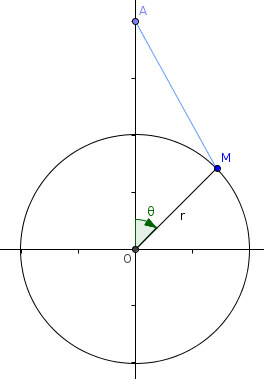
\includegraphics[scale=0.6]{Figures/sch1.png}
\end{figure}

% TODO expliquer démarche: nous avons utilisé la conservation de l'em pour trouver l'equation diff du système.

\subsection{Conservation de l'énergie mécanique}
L'énergie mécanique est la somme de l'énergie cinétique et de l'énergie potentielle. Celle-ci reste constante au cours du temps en l'absence de frottements. % TODO à compléter: parler de forces non-conservatives?

\begin{flalign*}
	Em &= Ep + Ec&\\
	   &= Epp + Epe + Ec,&
\end{flalign*}
avec $Em$ l'énergie mécanique, $Ep$ l'énergie potentielle, $Epp$ l'énergie potentielle de pesanteur, $Epe$ l'énergie potentielle élastique du ressort et $Ec$ l'énergie cinétique.

\paragraph{Énergie cinétique}
% TODO insérer brève définition

\begin{flalign*}
	Ec &= \frac{1}{2} m v^2 \text{, avec } v = r \dot{\theta}&\\
	   &= \frac{1}{2} m r^2 \dot{\theta}^2&
\end{flalign*}
\newpage

\paragraph{Énergie potentielle de pesanteur}\mbox{}\\
% TODO insérer brève définition

\begin{figure}[h]
	\centering
	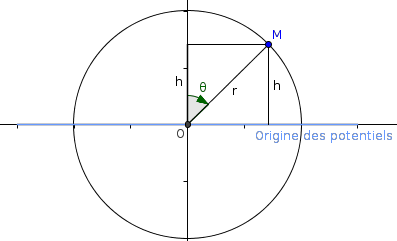
\includegraphics[scale=0.6]{Figures/sch2.png}
\end{figure}

\begin{align*}
   \left.\begin{array}{r@{\mskip\thickmuskip}l}
   \displaystyle
   \cos(\theta) = \frac{h}{r}\\
	h = r \cos(\theta)
  \end{array}
  \quad \right| \quad
  \begin{array}{r@{\mskip\thickmuskip}l}
    	Epp = mgh\\
	    = mgrcos(\theta)
  \end{array}
\end{align*}

\paragraph{Énergie potentielle élastique du ressort}
\begin{flalign*}
	&Epr = \frac{1}{2}k(l -l_0)&
\end{flalign*}
avec $l_0$: longueur du ressort au repos, $l$: longueur du ressort et $k$: constante de raideur du ressort.\\

\begin{multicols}{2}
\begingroup
	\centering
	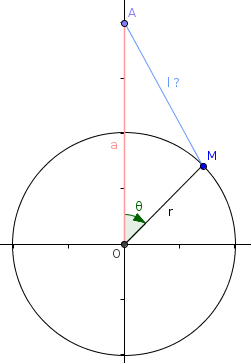
\includegraphics[scale=0.6]{Figures/sch3.png}
\endgroup

\underline{Théorème d'Al-Kashi}:
\begin{leftbar}
$\alpha$, $\beta$, $\gamma$ angles\\
a, b, c côtés opposés\\
$c^2 = a^2 + b^2 - 2ab\cos\gamma$
\end{leftbar}

Dans notre cas (voir figure ci-contre) :
\begin{flalign*}
l^2 &= a^2 + r^2 - 2ar\cos\theta&\\
l &= \sqrt{a^2 + r^2 - 2ar\cos\theta}&\\
Epr &= \frac{1}{2} k (\sqrt{a^2 + r^2 - 2ar\cos\theta} - l_0)^2&
\end{flalign*}
\end{multicols}

\paragraph{Intégrale première}
\begin{flalign*}
	Em &= Epp + Epe + Ec&\\
	   &= \frac{1}{2}mr^2 \dot{\theta}^2
	      + mgr\cos\theta
	      + \frac{1}{2}k \left(\sqrt{a^2 + r^2 - 2ar\cos\theta} - l_0\right)^2&
\end{flalign*}

\underline{On divise par $mr^2$} :
\begin{flalign*}
\frac{Em}{mr^2} &= \frac{1}{2} \dot{\theta}^2
                   + \frac{g}{r}\cos\theta
                   + \frac{1}{2} \frac{k}{mr^2}
                     \left(
                   		\sqrt{a^2 + r^2 - 2ar\cos\theta} - l_0
                   	 \right)^2&
\end{flalign*}

\underline{$g=r=l_0$ et $\frac{k}{m}=\frac{\lambda}{\mu}$} :
\begin{flalign*}
	\frac{Em}{mr^2} &= \frac{1}{2} \dot{\theta}^2
	                   + \cos\theta
	                   + \frac{1}{2}\frac{k}{mr^2}
	                    \left(
	                   		r\sqrt{\frac{a^2}{r^2} + 1 - 2\frac{a}{r}\cos\theta} - r
	                   	\right)^2&\\
	&= \frac{1}{2} \dot{\theta}^2
	   + \cos\theta
	   + \frac{1}{2} \frac{k}{m}
	     \left(
	   		\sqrt{\frac{a^2}{r^2} + 1 - 2\frac{a}{r}\cos\theta} - 1
	   	\right)^2&
\end{flalign*}

\begin{flalign*}
	&\boxed{
		\frac{Em}{mr^2} = \frac{1}{2} \dot{\theta}^2
		                  + \cos\theta
		                  + \frac{1}{2} \frac{\lambda}{\mu}
		                    \left(
		                  		\sqrt{\mu^2 + 1 - 2\mu\cos\theta} - 1
		                  	\right)^2
	}&
\end{flalign*}

$\displaystyle C = \frac{1}{2} \dot{\theta}^2 + H(\theta)$ avec
$\begin{cases}
	C = \frac{Em}{mr^2}\\
	H(\theta) = \cos(\theta) + \frac{1}{2} \frac{\lambda}{\mu} (\sqrt{\mu^2 + 1 - 2\mu\cos(\theta)} - 1)^2
\end{cases}$

\paragraph{Équation différentielle}\mbox{}\\
Pour trouver l'équation différentielle, il faut dériver l'intégrale première trouvée précédemment.

\begin{flalign*}
	C &= \frac{1}{2}\dot{\theta}^2 + H(\theta)&\\
	0 &= \frac{1}{2} \frac{\mathd}{\mathd t}\dot{\theta}^2 + \frac{\mathd}{\mathd t}H(\theta)&\\
	&= \ddot{\theta}\dot{\theta} + \dot{\theta} \frac{\mathd}{\mathd \theta}H(\theta)&\\
	&= \ddot{\theta} + \frac{\mathd}{\mathd \theta}H(\theta)&\\
	&= \ddot{\theta} + \frac{\mathd}{\mathd \theta}\left( \cos(\theta) + \frac{1}{2} \frac{\lambda}{\mu} (\sqrt{\mu^2 + 1 - 2\mu\cos\theta} - 1)^2 \right)&\\
	&= \ddot{\theta} -\sin\theta + \frac{1}{2}\frac{\lambda}{\mu}\frac{\mathd}{\mathd \theta}\left( (\sqrt{\mu^2 + 1 - 2\mu\cos\theta} - 1)^2 \right)&\\
	&= \ddot{\theta} -\sin\theta + \frac{1}{2}\frac{\lambda}{\mu}\frac{\mathd}{\mathd \theta}\left( f(\theta)^2 \right)&\\
	&= \ddot{\theta} -\sin\theta + \frac{\lambda}{\mu}f'(\theta)f(\theta)&\\
	&= \ddot{\theta} - \sin\theta + \frac{\lambda}{\mu} \left(
		\mu \sin(\theta) - \frac{\mu \sin\theta}{\sqrt{\mu^2 +1 -2\mu \cos\theta}}
	\right)&
\end{flalign*}

\begin{flalign*}
	&\boxed{
		0 = \ddot{\theta}
		    + \sin\theta
		      \left(
		      	-1 +\lambda
		    	- \frac{\lambda}{\sqrt{\mu^2 +1 -2\mu \cos\theta}}
		      \right)
	}&
\end{flalign*}

$\displaystyle  \ddot{\theta} + h(\mu,\lambda ; \theta) = 0$ avec
$\begin{cases}
	h(\mu,\lambda ; \theta) = \sin\theta\left(-1 +\lambda -\frac{\lambda}{\sqrt{\mu^2 +1 -2\mu \cos\theta}} \right)\\
	\lambda > 0\\
	\mu > 0
\end{cases}$

\newpage
\section{Cas sans frottement}
\subsection{Points d'équilibre}
% TODO insérer brève définition

Soit $\displaystyle h(\theta) = \sin\theta\left(-1 +\lambda -\frac{\lambda}{\sqrt{\mu^2 +1 -2\mu \cos\theta}} \right)$, si $h(\theta^*) = 0$, le point $\theta^*$ est un point d'équilibre du système.

\begin{flalign*}
	&\begin{cases}
		\sin\theta^* = 0\\
		-1 +\lambda -\frac{\lambda}{\sqrt{\mu^2 +1 -2\mu \cos\theta^*}} = 0
	\end{cases}&
\end{flalign*}

\paragraph{Premier cas}
\begin{flalign*}
	\sin\theta^* &= 0&\\
	\theta^* &= k\pi, \text{ avec } k\in\mathbb{N} &
\end{flalign*}
Le système possède donc au moins deux points d'équilibres (qui se répètent), $\theta^* = 0$ et $\theta^* = \pi$.

\paragraph{Second cas}
\begin{flalign*}
	-1 +\lambda -\frac{\lambda}{\sqrt{\mu^2 +1 -2\mu \cos\theta^*}} &= 0&\\
	\frac{\lambda}{\sqrt{\mu^2 +1 -2\mu \cos\theta^*}} &= \lambda - 1&\\
	\frac{1}{\sqrt{\mu^2 +1 -2\mu \cos\theta^*}} &= \frac{\lambda - 1}{\lambda}&\\
	\mu^2 +1 -2\mu \cos\theta^* &= \left(\frac{\lambda}{\lambda - 1}\right)^2&\\
	\cos\theta^* &= -\left(\left(\frac{\lambda}{\lambda - 1}\right)^2 -\mu^2 -1\right)\frac{1}{2\mu}&\\
\end{flalign*}
Si l'on peut résoudre l'équation si dessus, le système aura deux points d'équilibre supplémentaires ($\cos(\theta) = \cos(-\theta)$ ).\\

Recherche des cas limites pour $\cos\theta^* = -\left(\left(\frac{\lambda}{\lambda - 1}\right)^2 -\mu^2 -1\right)\frac{1}{2\mu}$, afin de connaître le nombre de points d'équilibre pour $\lambda$ fixé en fonction de $\mu$.

\begin{flalign*}
	&\begin{cases}
		-\left(\left(\frac{\lambda}{\lambda - 1}\right)^2 -\mu^2 -1\right)\frac{1}{2\mu} > -1& (1)\\
		-\left(\left(\frac{\lambda}{\lambda - 1}\right)^2 -\mu^2 -1\right)\frac{1}{2\mu} < 1& (2)
	\end{cases}&
\end{flalign*}

\underline{Résolution de (1)}:
\begin{flalign*}
	-\left(\left(\frac{\lambda}{\lambda - 1}\right)^2 -\mu^2 -1\right)\frac{1}{2\mu} &> -1&\\
	\left(\frac{\lambda}{\lambda - 1}\right)^2 -\mu^2 -1 &> 2\mu&\\
	\left(\frac{\lambda}{\lambda - 1}\right)^2 -\mu^2 -1 - 2\mu &> 0&\\
	\left(\frac{\lambda}{\lambda - 1}\right)^2 - (\mu + 1)^2 &> 0&\\
	\left(\frac{\lambda}{\lambda - 1} -\mu -1\right)\left(\frac{\lambda}{\lambda - 1} +\mu +1\right) &> 0&\\
\end{flalign*}

$\Rightarrow \mu > \frac{\lambda}{\lambda -1} - 1$ ou $\mu > -\frac{\lambda}{\lambda -1} - 1$\\

\underline{Résolution de (2)}:
\begin{flalign*}
	-\left(\left(\frac{\lambda}{\lambda - 1}\right)^2 -\mu^2 -1\right)\frac{1}{2\mu} &< 1&\\
	\left(\frac{\lambda}{\lambda - 1}\right)^2 -\mu^2 -1 &< -2\mu&\\
	%
	\left(\frac{\lambda}{\lambda - 1}\right)^2 - (\mu - 1)^2 &< 0&\\
	\left(\frac{\lambda}{\lambda - 1} -\mu +1\right)\left(\frac{\lambda}{\lambda - 1} +\mu -1\right) &< 0&\\
\end{flalign*}

$\Rightarrow \mu < \frac{\lambda}{\lambda -1} + 1$ ou $\mu < -\frac{\lambda}{\lambda -1} + 1$\\

\underline{(1) et (2)}:\\

$\mu > 0$ et $\lambda > 0$, donc $\boxed{\displaystyle \mu \in \left] \frac{\lambda}{\lambda - 1}-1 ; \frac{\lambda}{\lambda - 1}+1 \right[}$.\\

Application numérique pour $\lambda = 2$ : $\mu \in ]1;3[$.

\paragraph{Conclusion} \mbox{}\\
Le système possède au moins deux points d'équilibre: $\theta^* = 0$ et $\theta^* = \pi$, et au plus 4 points d'équilibre si $\displaystyle \mu \in \left] \frac{\lambda}{\lambda - 1}-1 ; \frac{\lambda}{\lambda - 1}+1 \right[$. Ces points d'équilibre peuvent être stables ou instables, et il y a alternance entre stabilité et instabilité.

\newpage
\paragraph{Matlab} \mbox{}\\
\begin{figure}[h!]
	\centering
	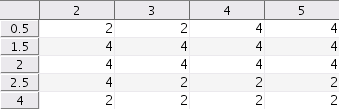
\includegraphics[scale=0.65]{Figures/rapport_nbequi.png}
	\caption{Nombre de points d'équilibre en fonction de $\lambda$ (colonnes) et $\mu$ (lignes)}
\end{figure}

\begin{lstlisting}
function pr3001_B
	lambda_vector=[1 2 3 4 5];
	mu=[0.5 1.5 2 2.5 4];
	...
	displayNbEqui(lambda_vector, mu);
	...
end

% Affiche le nombre de points d'équilibres en fonction de lambda et mu dans
% un tableau.
function displayNbEqui(lambda, mu)
    Z = nbEqui(lambda, mu);
    
    f = figure('name', 'Nombre de points d''équilibre(lambda, mu)', 'Position', [0 0 600 350]);
    t = uitable('Parent', f, 'Position', [50 700 500 150]);
    set(t, 'Data', Z, 'ColumnName', lambda, 'RowName', mu)
end

% Calcul le nombre de points d'équilibres pour chaque lambda et mu
% (vecteurs). Retourne une matrice (ligne: taille de lambda, colonne: taille de 
% mu).
function z=nbEqui(lambda, mu)
    z = zeros(length(lambda), length(mu));
    
    for i=lambda
        for j=1:length(mu)
            if (mu(j) < (lambda(i)/(lambda(i)-1)) + 1) && (mu(j) > (lambda(i)/(lambda(i)-1)) - 1)
                z(i,j) = 4;
            else
                z(i,j) = 2;
            end
        end
    end
end
\end{lstlisting}
La fonction \emph{nbEqui} vérifie la condition $\displaystyle \mu \in \left] \frac{\lambda}{\lambda - 1}-1 ; \frac{\lambda}{\lambda - 1}+1 \right[$ et remplit un tableau à 2 dimensions en fonction de $\lambda$ et $\mu$. A chaque couple de $\lambda$ et $\mu$ est associé un nombre de points d'équilibre. La fonction \emph{displayNbEqui} affiche ensuite le tableau dans l'ui.

% TODO insérer code + explications

\newpage
\subsection{Portrait de phase}
\begin{figure}[h!]
	\centering
	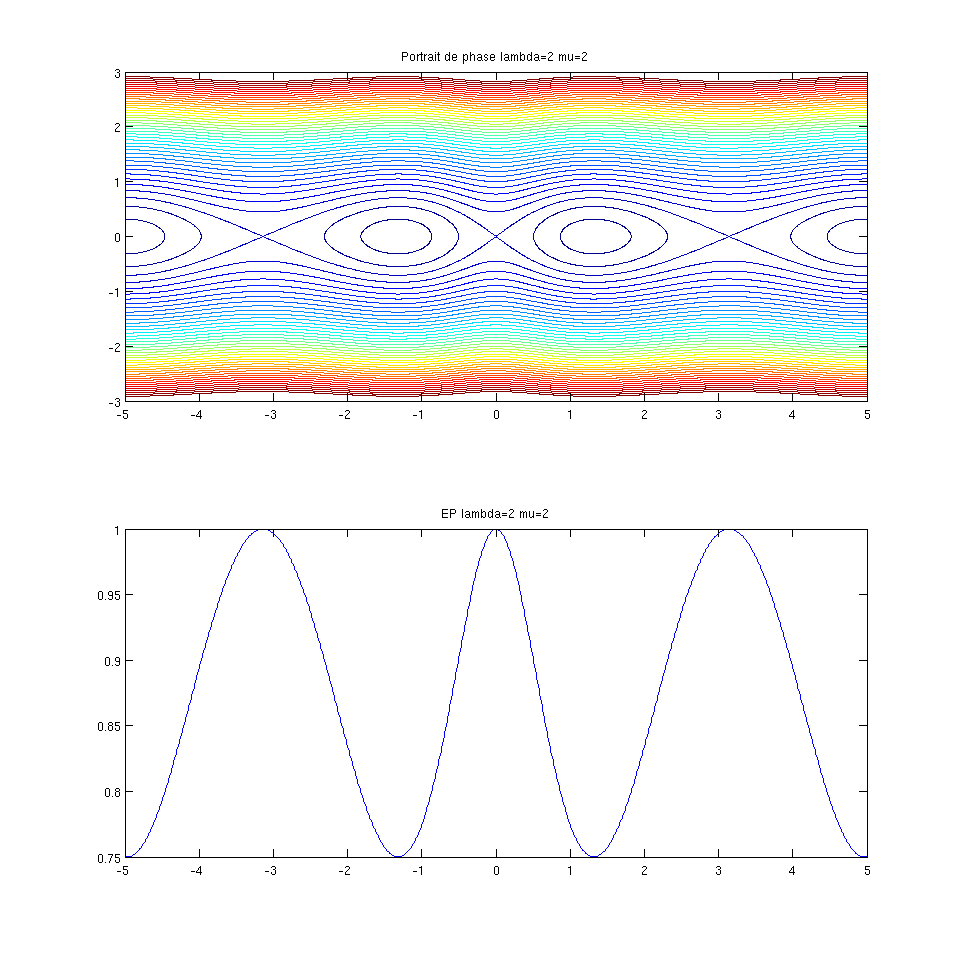
\includegraphics[scale=0.65]{Figures/rapport_figportraitphasemu2.png}
	\caption{Portrait de phase (haut) et énergie potentielle (bas) pour $\lambda=2$ et $\mu=2$}
\end{figure}

Le portrait de phase représente différentes trajectoires possibles pour le système dans le plan de phase $(\theta,\dot{\theta})$. A chaque couple de conditions initiales $(\theta_0, \omega_0)$ est associée une trajectoire différente.
% TODO LIRE DOC Thweatt1999.pdf : décrire allure mouvement oscillatoire (courbes fermés) vs mouvement révolutif (courbes ouvertes), séparatrice
% TODO dire pourquoi mu=1 a été exclu (on ne peut pas avoir de ressort ponctuel)
% TODO insérer figures rapport_figportraitphasemu2
% TODO interprétation des portraits de phase (notamment le nombre de points d'équilibre)
% TODO insérer code + explications

\paragraph{Matlab}
\newpage

\subsection{Vitesse initiale maximale pour une trajectoire périodique}
Nous souhaitons obtenir la vitesse initiale maximale pour une trajectoire périodique sachant que nous avons fixé la position $x_0$ à $\frac{\pi}{2}$. La séparatrice est la limite entre les trajectoires décrivant un mouvement oscillatoire et les trajectoires décrivant un mouvement révolutif. Celle-ci relie les points d'équilibres instable. % TODO à compléter
Nous cherchons donc l'intersection entre la trajectoire séparatrice et $\frac{\pi}{2}$. La trajectoire séparatrice qui nous intéresse passe par un des 2 points d'équilibres suivants (voir les deux) : $0$ et $\pi$.
\begin{flalign*}
	C &= \frac{1}{2} \dot{\theta}^2 + H(\theta)&\\
	\dot{\theta} &= \sqrt{2(C - H(\theta))}
\end{flalign*}

\underline{$\lambda = 2$, $\theta_0=\frac{\pi}{2}$}:
\begin{flalign*}
	\dot{\theta} &= \sqrt{2\left( C - \frac{1}{\mu}\left( \sqrt(\mu^2 + 1) - 1 \right)^2 \right)}&
\end{flalign*}

\underline{Aux points d'équilibre $\theta^*=0$ et $\theta^* = \pi$} :\\
L'énergie mécanique est égale à l'énergie potentielle, en effet la vitesse est nulle aux points d'équilibres, l'énergie cinétique y est donc nulle. Cela nous donne donc $C = H(\theta^*)$.
\begin{flalign*}
	C = H(\theta^*) &= \frac{1}{\mu}\left( \sqrt{\mu^2 +1 -2\mu\cos\theta^*} -1 \right)^2 + cos \theta^*&\\
	H(0) &= \frac{1}{\mu}\left( \sqrt(\mu^2 + 1 -2\mu) - 1 \right)^2 + 1&\\
	H(\pi) &= \frac{1}{\mu}\left( \sqrt(\mu^2 + 1 +2\mu) - 1 \right)^2 - 1&
\end{flalign*}

\begin{leftbar}
	\textbf{N.B.} $H(0) \neq H(\pi)$ sauf pour $\mu=2$ :
	\begin{flalign*}
		\frac{1}{\mu}\left( \sqrt(\mu^2 + 1 -2\mu) - 1 \right)^2 + 1 &= \frac{1}{\mu}\left( \sqrt(\mu^2 + 1 +2\mu) - 1 \right)^2 - 1&\\
		\frac{\mu^2 -\mu -2\sqrt{\mu^2 + 1 -2\mu} +2}{\mu} &= \frac{\mu^2 + \mu -2\sqrt{\mu^2 + 1 + 2\mu} + 2}{\mu}&\\
		-\mu -2\sqrt{(-1 + \mu)^2} &= \mu -2\sqrt{(1 + \mu)^2}&\\
		\mu &= 2 \quad\quad (\mu = \pm 2 \text{, mais } \mu>0)&
	\end{flalign*}
	Pour $\mu=2$, la séparatrice passe par les deux points d'équilibre $\theta^*=0$ et $\theta^*=\pi$.
\end{leftbar}

On s'intéresse au final à la trajectoire qui passe par le point d'équilibre ($\theta^*=0$ ou $\theta^*=\pi$) dont l'énergie est la plus élevée.

\begin{leftbar}
\textbf{Exemple :} $\mu = 4$
\begin{flalign*}
	H(0) &= \frac{1}{4}\left( \sqrt{4^2 + 1 -2*4} - 1 \right)^2 + 1 = 2&\\
	H(\pi) &= \frac{1}{4}\left( \sqrt{4^2 + 1 +2*4} - 1 \right)^2 - 1 = 3&\\
	H(\pi) &> H(0)&
\end{flalign*}
\begin{flalign*}
	C &= H(\pi) = 3 \text{, de plus}\\
	C &= \frac{1}{2}\dot{\theta}^2 + \frac{1}{\mu}\left( \sqrt{\mu^2 + 1} -1 \right)^2&\\
	\omega_{0max} &= \sqrt{2\left( \left( C - \frac{1}{\mu}\left( \sqrt{\mu^2 + 1} - 1 \right) \right)^2\right)} = 1.0598&
\end{flalign*}
\end{leftbar}

\begin{figure}[h!]
	\centering
	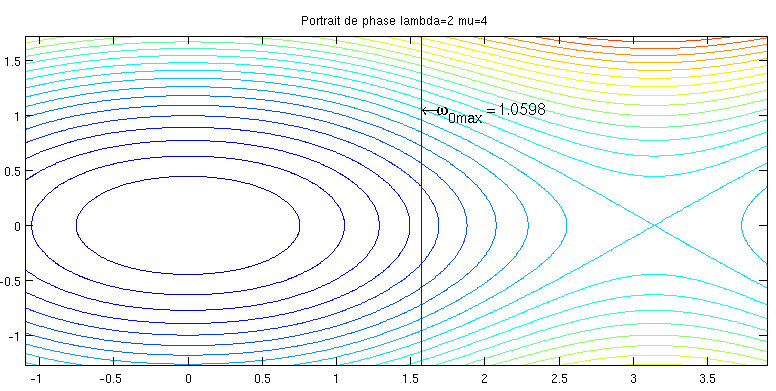
\includegraphics[scale=0.65]{Figures/rapport_figomega0.png}
	\caption{$\omega_{0max}$ sur le portrait de phase pour $\lambda = 2$ et $\mu = 4$}
\end{figure}

\paragraph{Matlab}\mbox{}\\
Le programme suivant permet d'afficher la position du point $(\theta_0,\omega_{0max})$ sur le portrait de phase.
Pour cela, à chaque $\mu$ la valeur de  $\omega_{0max}$ est calculée à l'aide de la fonction \emph{vitesseInitMax}, puis on positionne le point sur le portrait de phase à l'aide de la fonction \emph{text}.\\
La fonction \emph{vitesseInitMax} calcule la vitesse angulaire (fonction \emph{vitesseAngulaire}) aux $\lambda$, $\mu$, $\theta_0$ donnés et à l'aide de C, sachant que C a pour valeur le maximum entre $H(0)$ et $H(\pi)$.

\begin{lstlisting}
function pr3001_B
    ...
    lambda=2;
    mu=[0.5 1.5 2 2.5 4];
    x0=pi/2;
    ...

    for i=mu
        figure
        subplot(2,1,1)
        portraitPhase(lambda, i);
        w0max=vitesseInitMax(lambda, i, x0);
        line([x0 x0], [-5 5])
        str=strcat('\leftarrow\omega_{0max} = ', num2str(w0max));
        text(x0, w0max, str, 'FontSize', 14)
        ...
    end
end

function z=vitesseAngulaire(lambda, mu, C, x)
    z=sqrt(2*(C - H_IntegPrem(lambda, mu, x)));
end

% Calcul de la valeur max de la vitesse initiale w0 pour laquelle la
% trajectoire est périodique, sachant que l'on fixe la position initiale
% x0, lambda et mu.
function w0max=vitesseInitMax(lambda, mu, x0)
    H0=H_IntegPrem(lambda, mu, 0);
    Hpi=H_IntegPrem(lambda, mu, pi);
    if H0 > Hpi
        C=H0;
    else
        C=Hpi;
    end

    w0max=vitesseAngulaire(lambda, mu, C, x0);
end
\end{lstlisting}
\newpage

\subsection{Mouvement et période}
\newpage

\appendix
\section{Annexe: portraits de phase}
\begin{figure}[h!]
	\centering
	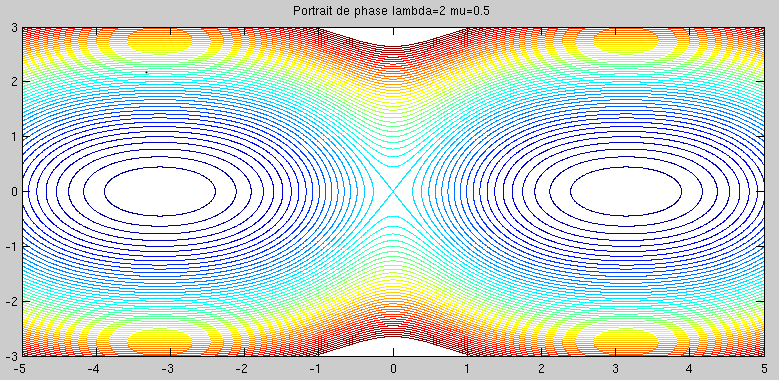
\includegraphics[scale=0.64]{Figures/rapport_pp05.png}
\end{figure}

\begin{figure}[h!]
	\centering
	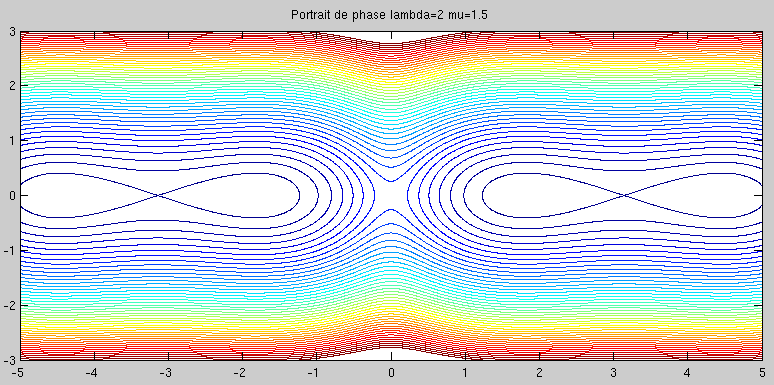
\includegraphics[scale=0.65]{Figures/rapport_pp15.png}
\end{figure}

\begin{figure}[h!]
	\centering
	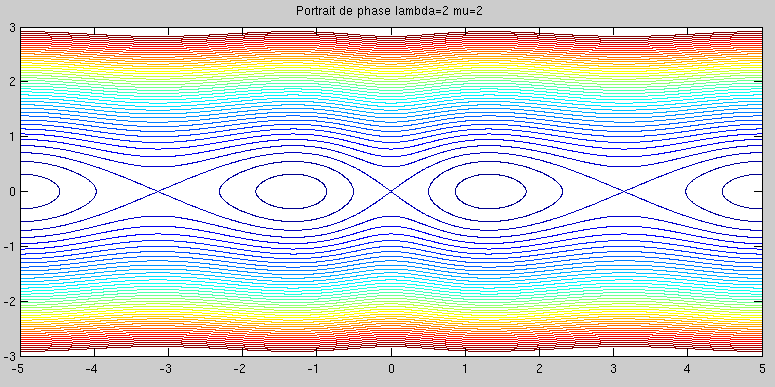
\includegraphics[scale=0.65]{Figures/rapport_pp20.png}
\end{figure}

\begin{figure}[h!]
	\centering
	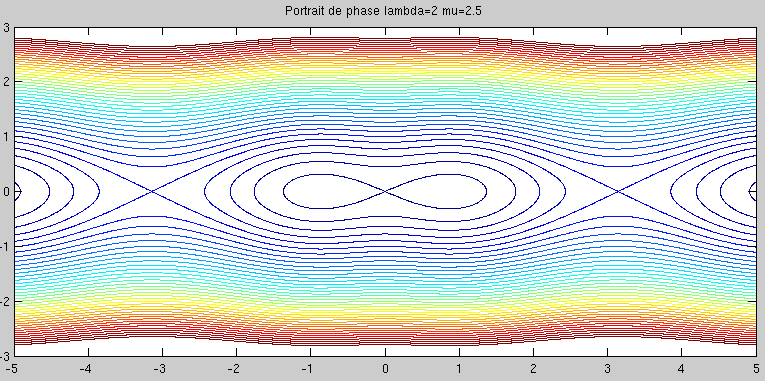
\includegraphics[scale=0.66]{Figures/rapport_pp25.png}
\end{figure}

\begin{figure}[h!]
	\centering
	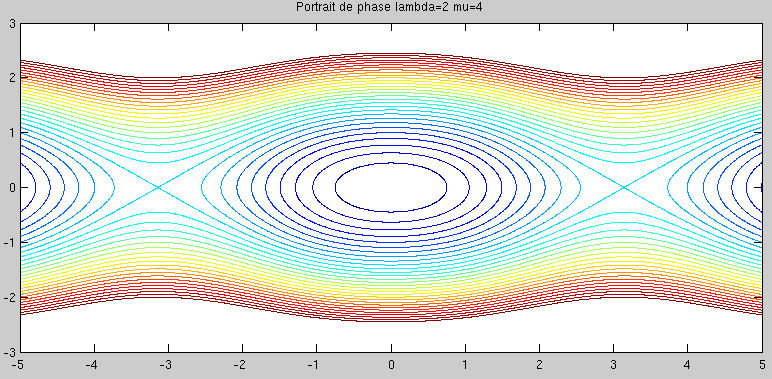
\includegraphics[scale=0.65]{Figures/rapport_pp40.png}
\end{figure}

\end{document}
